\section{Results}\label{sec:b-results}

\subsection{RQ1: Faithfulness}
The static trace matches what Qiskit builds. On all \numToolDevPrograms{} of our runnable programs, of up to
\numToolDevMaxOps{} operations, the trace equals the circuit the program builds when it runs, and on all
\numQasmCircuitsChecked{} benchmark circuits the OpenQASM reader's trace equals the circuit Qiskit loads. The slices match
the light cone of the built circuit on \numToolDevSliceEqual{} of the programs. The remaining one nests one condition
inside another, which the reference slicer on the circuit reads by the outer condition only, while \tool{} follows the
bits of both, so there \tool{} is the more precise of the two. On all \numToolTTwoUnits{} Bugs4Q units whose operations map
to lines, \tool{}'s line slices equal those recorded while the ported programs run.

Loops that run on the device are sliced soundly. In the \numCfPrograms{} programs with device loops, branches and
switches, deleting every operation outside a qubit's slice from the source leaves the state of each of the
\numCfQubits{} qubits unchanged at \numCfInputs{} inputs under exact simulation, as Proposition~\ref{prop:b-loops}
predicts, while slices that read each loop body once are wrong on \numCfOldWrong{} of the \numCfPrograms{} programs.

The classical statements are where the approach is least exact. srcSlice's lines contain those of the flow-sensitive
reference for \numSsContainPct{} of \numSsQubits{} qubits in \numSsFiles{} files, and for \numSsDevBugsContainPct{} on our
programs and Bugs4Q, but for only \numSsHeldContainPct{} on the \numSsHeldFiles{} held-out programs of LintQ's corpus. Most
misses lie in functions that build a value and return it, which srcSlice's forward slices do not link to the call, so
\tool{} shows both sets of classical lines.

\emph{Answer to RQ1.} Without running a program, \tool{} reconstructs the circuit it builds and slices it as the light
cone of the built circuit does, device loops included. Its classical statements are complete for most qubits but miss
values returned from functions in held-out code.

\subsection{RQ2: Coverage}
Of the \numScaleSOneFiles{} programs of LintQ's corpus, \tool{} traces a circuit in \numScaleSOneSliced{}. Of the
\numCovNoCircuit{} that yield none, \numCovNoConstruction{} never construct a circuit, such as helpers and scripts that
read results, \numCovFromFile{} load their circuits from a file or a library, and \numCovOther{} build them in code the
interpretation does not follow. It traces \numSubjBugsTraced{} of the \numSubjBugsCount{} Bugs4Q programs and
\numSubjTextTraced{} of the \numSubjTextCount{} textbook programs. On current Qiskit, it traces \numQheTracedOfBuildsPct{}
of the \numQheBuilds{} Qiskit HumanEval programs that construct a circuit. Where tracing stops, the cause is mostly a
method outside the role table. \numUnmodMethodProgs{} programs of LintQ's corpus call one, most often a method that runs
or simulates the circuit, such as \texttt{run}, or builds it from text, and otherwise operations such as
\texttt{reverse\_bits}, or \texttt{prepare\_state} in \numUnmodQhePrepare{} Qiskit HumanEval programs. Adding such methods
is the main way to widen coverage.

\emph{Answer to RQ2.} The approach slices most programs that build a circuit in code, and its failures are reported
with a cause, most often a method it does not yet model.

\subsection{RQ3: Cost and scalability}

\begin{figure}[t]
  \centering
  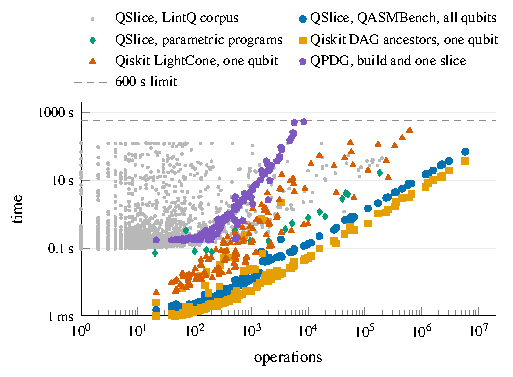
\includegraphics[width=\columnwidth]{figures/fig_scale_anon.pdf}% camera-ready: fig_scale.pdf, which names the tool
  \caption{Time of \tool{} against the operations of a trace. Grey points are the programs of LintQ's corpus, with every
  stage. The QASMBench points slice every qubit in one pass, reading included, and the baselines slice one qubit of the
  same circuits, loading included. Runs beyond the 600~s limit are left out.}
  \label{fig:b-scale}
\end{figure}

\tool{} slices the programs developers write in milliseconds and circuits of millions of operations in seconds, as
Fig.~\ref{fig:b-scale} shows. On LintQ's corpus it slices the \numScaleSOneSliced{} programs that build a circuit, every
qubit up to 64 of them, in \numScaleSOneMedianMs{}~ms per program in the median and within \numScaleSOneNinetyNine{}~s
for 99\% of them, and \numScaleSOneTimeouts{} programs reach the limit of 120~s. srcML and srcSlice take most of the
median, \numScaleSOneSrcmlMs{} and \numScaleSOneSrcsliceMs{}~ms, and the slices themselves \numScaleSOneSliceMs{}~ms. On
the \numScaleQbRead{} QASMBench circuits in valid OpenQASM~2, of up to \numScaleQbMaxOps{} operations and
\numScaleQbMaxQubits{} qubits, slicing every qubit in one pass takes at most \numScaleQbAllS{}~s, on the largest circuit,
after \numScaleQbReadS{}~s of reading. Qiskit's DAG slices one of its \numScaleQbMaxOpsQubits{} qubits in
\numScaleQbDagOneS{}~s after \numScaleQbDagLoadS{}~s of loading, about \numScaleQbDagAllMin{} minutes for all of them.
Qubit for qubit the two are close, one \tool{} slice taking \numScaleOneRatio{} times Qiskit's in the median, so
\tool{}'s advantage on large circuits is the single pass over every qubit. The QPDG reimplementation builds its graph
within the limit for circuits of up to \numScaleQpdgMaxOps{} operations, in \numScaleQpdgMaxS{}~s, where \tool{} reads and
slices the circuit in \numScaleQpdgSqS{}~s. Qiskit's \texttt{LightCone} pass slices one qubit of the circuit of
\numScaleLcMaxOps{} operations in \numScaleLcMaxS{}~s, where \tool{} slices all \numScaleLcQubits{} of its qubits in
\numScaleLcSqS{}~s. On the parametric programs the source stays at about a dozen lines while the trace grows. The QFT on
600 qubits unrolls \numScaleQftOps{} operations from \numScaleQftLines{} code lines in \numScaleQftS{}~s, where running
the program with Qiskit and slicing one qubit takes \numScaleQftRunS{}~s, the speed a static slicer gives up so that it
never executes the program.

\emph{Answer to RQ3.} The approach takes a fraction of a second per real program and scales to circuits of millions of
operations, where its one pass over every qubit outpaces tools that slice one qubit of the built circuit.

\subsection{RQ4: What a slice shows}

\begin{table}[t]
  \centering
  \caption{Predicates on \tool{}'s qubit profiles at the lines of LintQ's warnings of its five qubit analyses}
  \label{tab:b-lintq}
  \footnotesize\setlength{\tabcolsep}{4pt}\renewcommand{\arraystretch}{1.12}
  \newcommand{\sep}{\arrayrulecolor{black!25}\hline\arrayrulecolor{black}}
  \begin{tabular}{@{}l r r r@{}}
    \toprule
    \textbf{Warnings} & \textbf{Count} & \textbf{Traced} & \textbf{Predicate holds} \\
    \midrule
    True positives, by LintQ's labels & \numLqQubitTp{} & \numLqQubitTraced{} & \numLqQubitExposed{} \\ \sep
    False positives, by LintQ's labels & \numLqFpWarnings{} & \numLqFpTraced{} & \numLqFpFires{} \\ \sep
    All warnings of these analyses & \numLqSarifWarnings{} & \numLqSarifTraced{} & \numLqSarifFires{} \\
    \bottomrule
  \end{tabular}\\[3pt]
  \begin{minipage}{\columnwidth}\footnotesize
  The analyses are operation after measurement, double measurement, oversized circuit, conditional without measurement
  and unmeasurable qubits.
  \end{minipage}
\end{table}

A slice narrows what a developer reads. A qubit's slice holds \numScaleReadMedianPct{} of a program's code lines in the
median over LintQ's corpus, together with the loop iterations that put each line there.

Slices answer a different question from a bug detector's, where to look rather than what is wrong, and the comparison
with LintQ asks what the qubit view adds to its warnings. Table~\ref{tab:b-lintq} shows that the profiles contain what
LintQ's qubit analyses check. Of the \numLqQubitTp{} warnings LintQ's authors labelled true positives, \tool{} traces
\numLqQubitTraced{}, and a predicate on the profiles holds at the warned line of all of them. The predicates also hold
on \numLqFpFires{} of the \numLqFpTraced{} traced warnings the authors labelled false positives, so the profiles reproduce
these analyses with their false alarms and are not a more precise detector. What they add is context. LintQ points to
one line, and the slices of the qubits on that line give the \numLqReadMedian{} lines in the median that determine their
state, out of \numLqCodeMedian{} code lines in the file. LintQ's bound of ten loop iterations also matters. In
\numLqBeyondTenFiles{} of the programs \tool{} traces, operations are created after the tenth iteration of a loop,
\numLqBeyondTenOpsPct{} of all their operations.

\emph{Answer to RQ4.} A slice asks a developer to read about a quarter of a program, and beside a bug detector it shows
the few lines that determine the qubits a warning names.
